\section{\lr{IO Cache}}
در این قسمت من از کامپیوتر شخصی خودم به جای لپتاپ استفاده کردم. در ابتدا 5 گیگابایت از
\lr{SSD}
که ویندوز بر روی آن نصب بود را خالی
(\lr{unallocated})
کردم که بتوانم آنرا در
\lr{openCAS}
به عنوان کش معرفی کنم. سپس 20 گیگابایت از هارد دیسک خودم را نیز خالی کردم که بتوانم آنرا به عنوان
\lr{backend device}
معرفی کنم. خود لینوکس نیز بر روی دیسکی که یک پارتیشن از آن را خالی کرده بودم قرار دارد.

با تمام این صحبت‌ها شروع به نصب و کامپیال
\lr{openCAS}
می‌کنیم. در ابتدا من داشتم سعی می‌کردم که بر روی کرنل
\lr{5.19}
آنرا نصب کنم اما متاسفانه موفق نشدم. به همین جهت با توجه به
\link{https://github.com/Open-CAS/open-cas-linux/releases/tag/v22.6.2}{\lr{release notes}}
آخرین ورژن
\lr{openCAS}
متوجه شدم که نوشته‌اند که مشکلاتی بر روی لینوکس
\lr{5.15}
را درست کرده‌اند. پس من با کرنل
\lr{5.15}
امتحان کردم و موفقیت آمیز بود. مراحل نصب را از
\link{https://open-cas.github.io/getting_started_open_cas_linux.html}{این لینک}
دنبال کردم. در شکل
\ref{fig:openCAS_compile}
می‌توانید مراحل آنرا ببینید.
\begin{figure}[H]
    \centering
    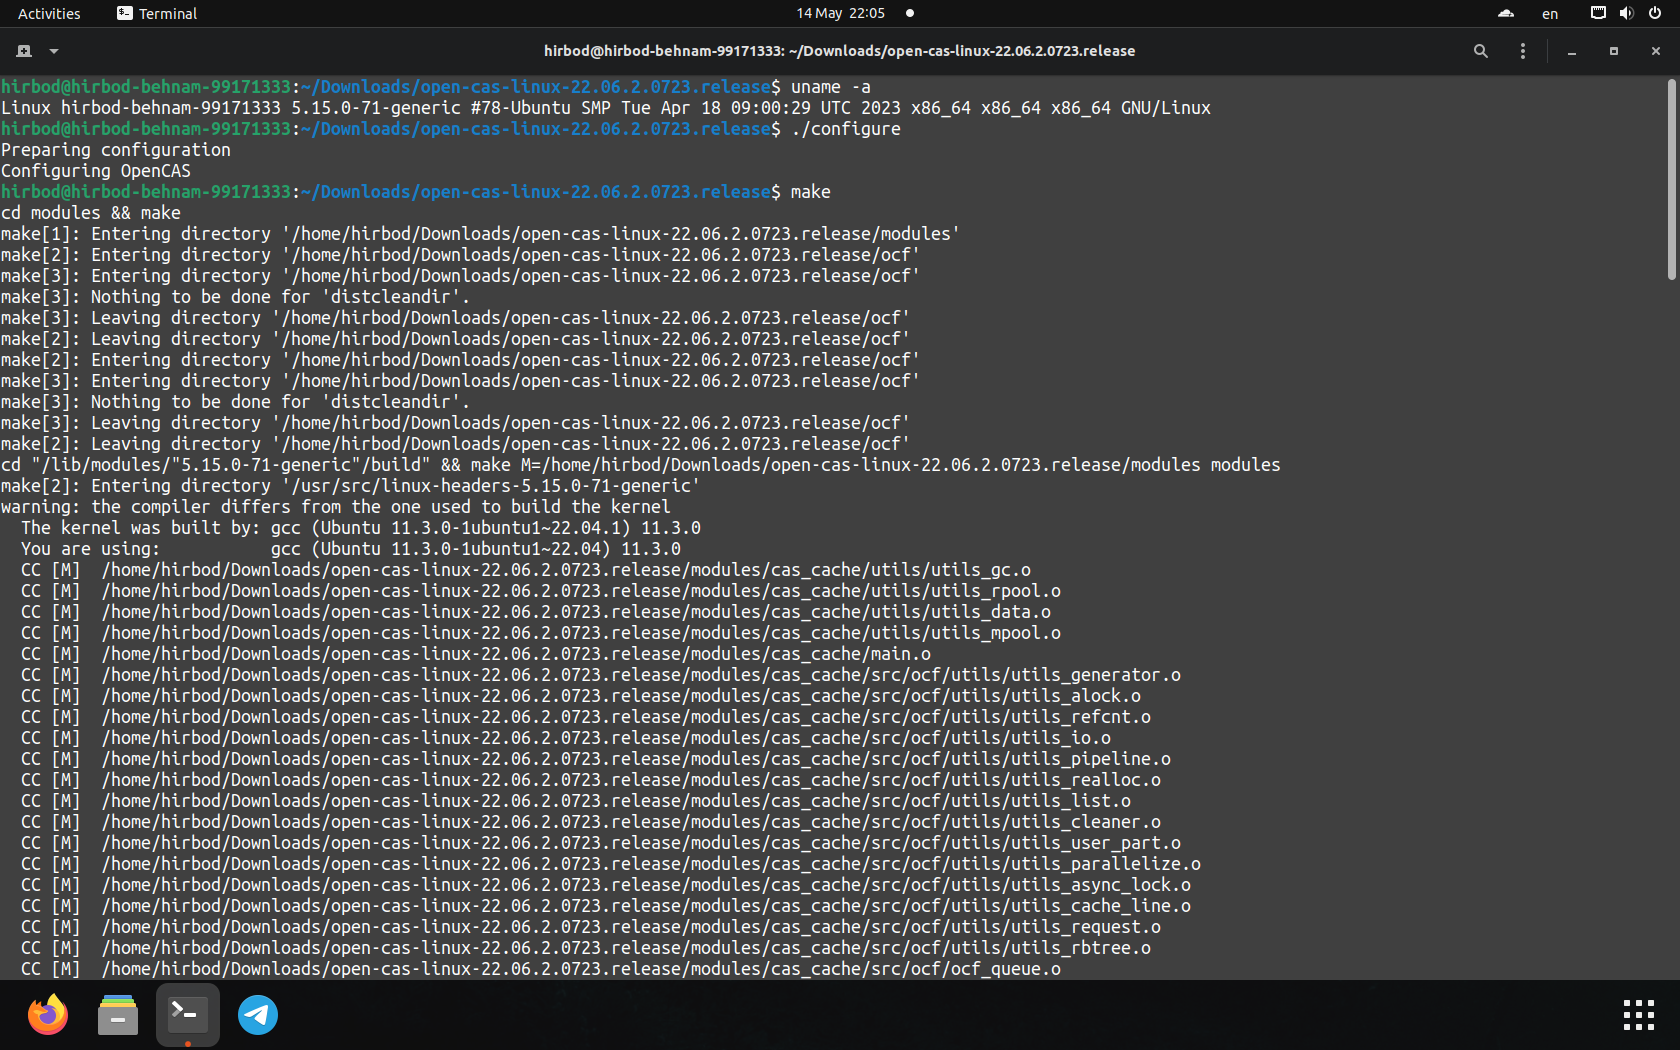
\includegraphics[scale=0.25]{pic/3-compile-1.png}
    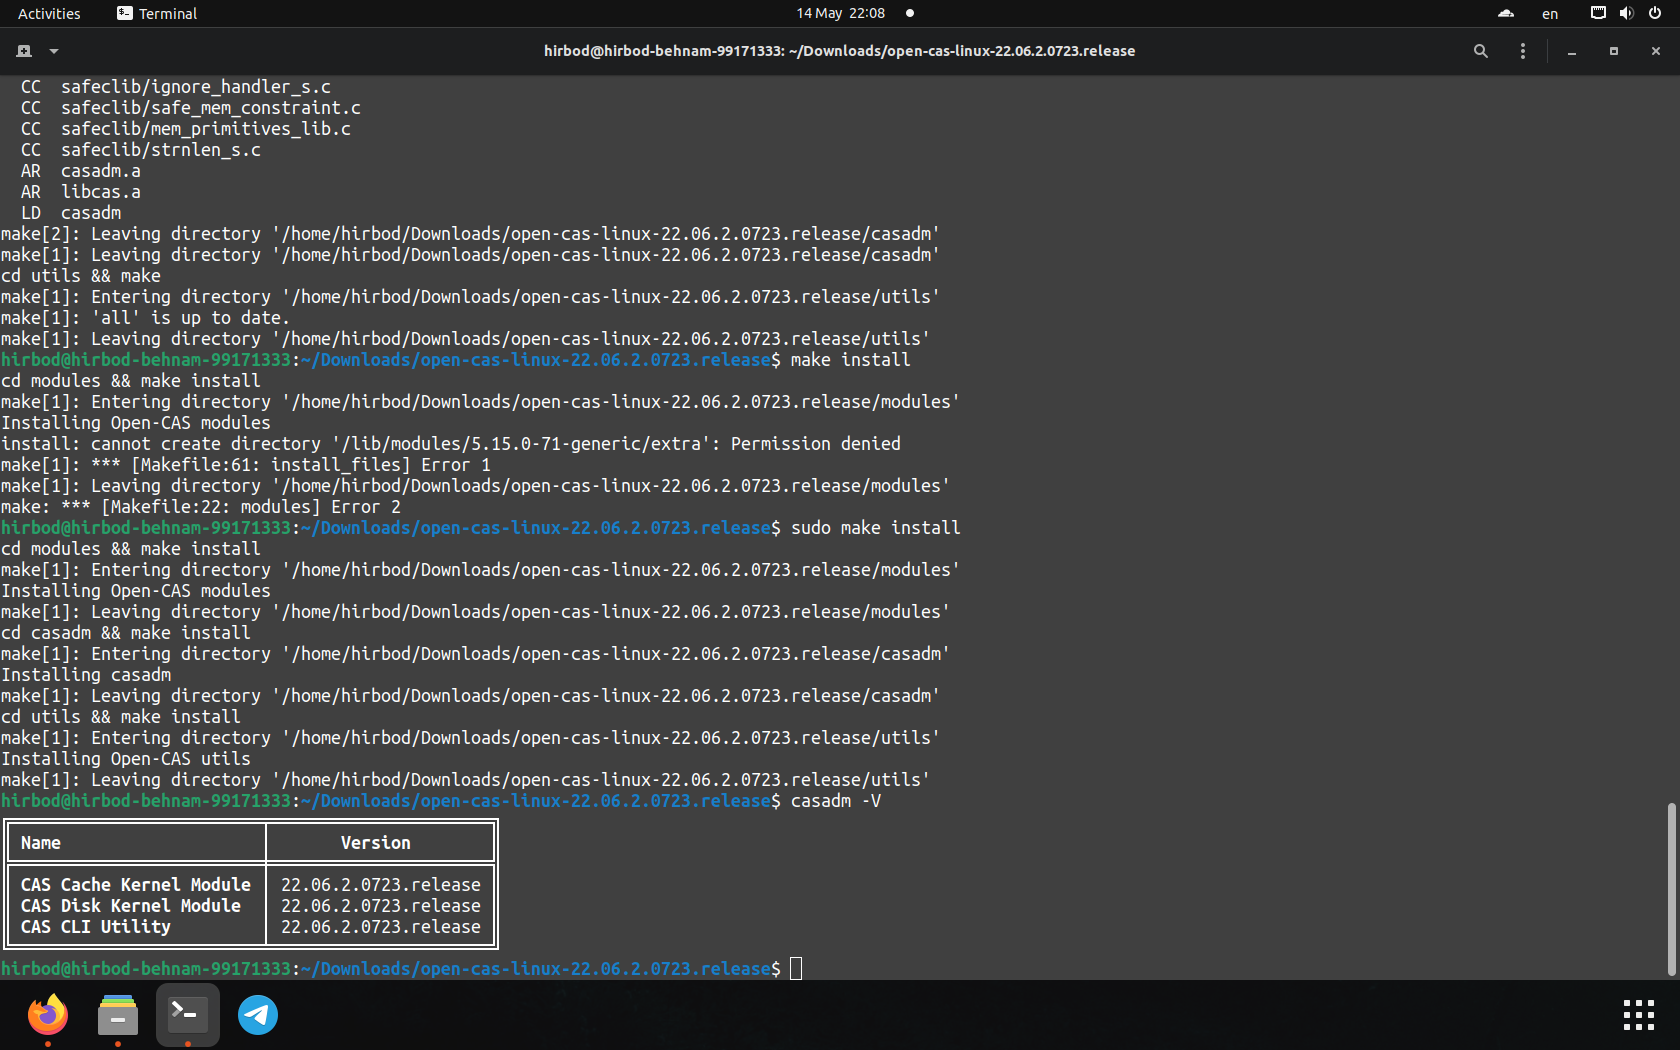
\includegraphics[scale=0.25]{pic/3-compile-2.png}
    \caption{کامپایل کردن \lr{openCAS}}
    \label{fig:openCAS_compile}
\end{figure}

سپس به کمک دستور زیر
(که در پوشه‌ی \lr{codes} کنار تمرین نیز موجود است)
برنامه را اجرا می‌کنیم. نتیجه‌ی اجرا در شکل
\ref{fig:3-1}
آمده است.
\samplebox{fio --filename="/media/hirbod/Linux External/file.txt" --direct=1 --rw=write --io\_size=20G --bs=4MB --ioengine=libaio --iodepth=8 --numjobs=1 --group\_reporting --size=20GB --name=iops\_test\_job --eta-newline=1 --output=seq-write-20.txt}
\begin{figure}[H]
    \centering
    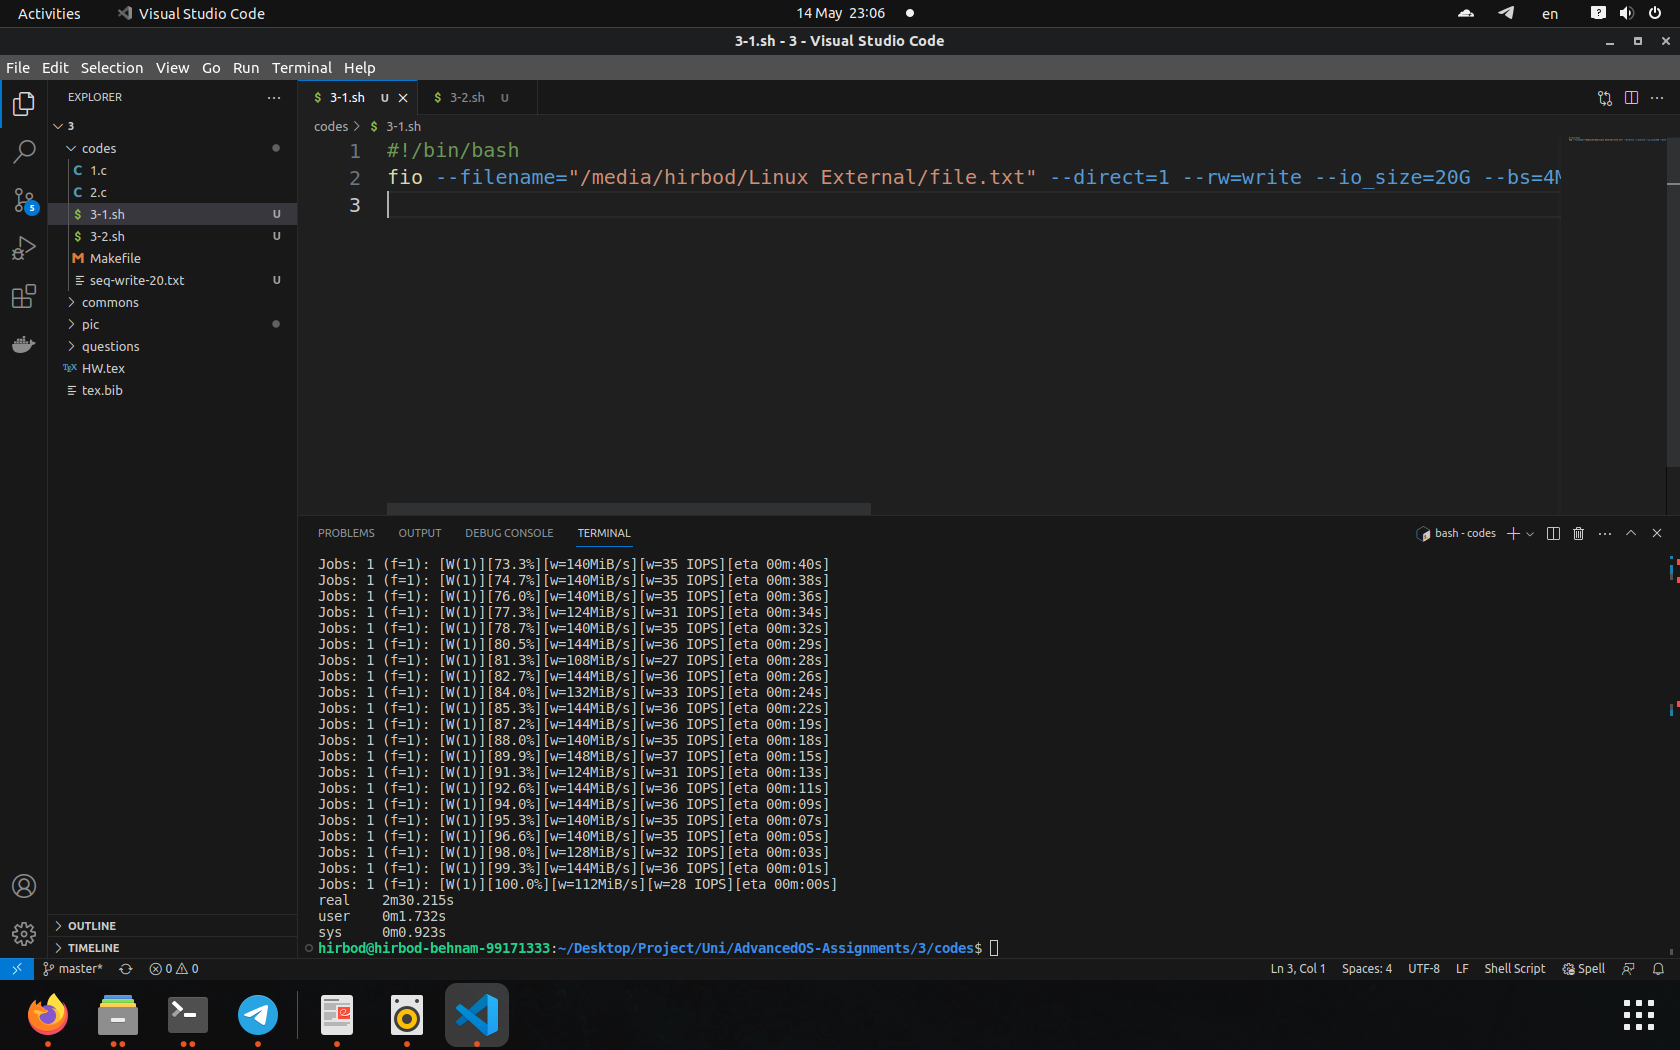
\includegraphics[scale=0.25]{pic/3-1.png}
    \caption{نوشتن فایل مستقیم در هارد}
    \label{fig:3-1}
\end{figure}

همچنین نتایج درست شده توسط
\codeword{fio}
را در فولدر
\lr{codes}
ببینید.

در ابتدا دستور قسمت دوم رو اجرا می‌کنیم:
\samplebox{fio --filename="/media/hirbod/Linux External/file.txt" --random\_distribution=zipf:1.2 --direct=1 --rw=read --io\_size=20G --bs=4MB --ioengine=libaio --iodepth=8 --numjobs=1 --group\_reporting --size=20GB --name=iops\_test\_job --eta-newline=1 --output=seq-read-20.txt}
\begin{figure}[H]
    \centering
    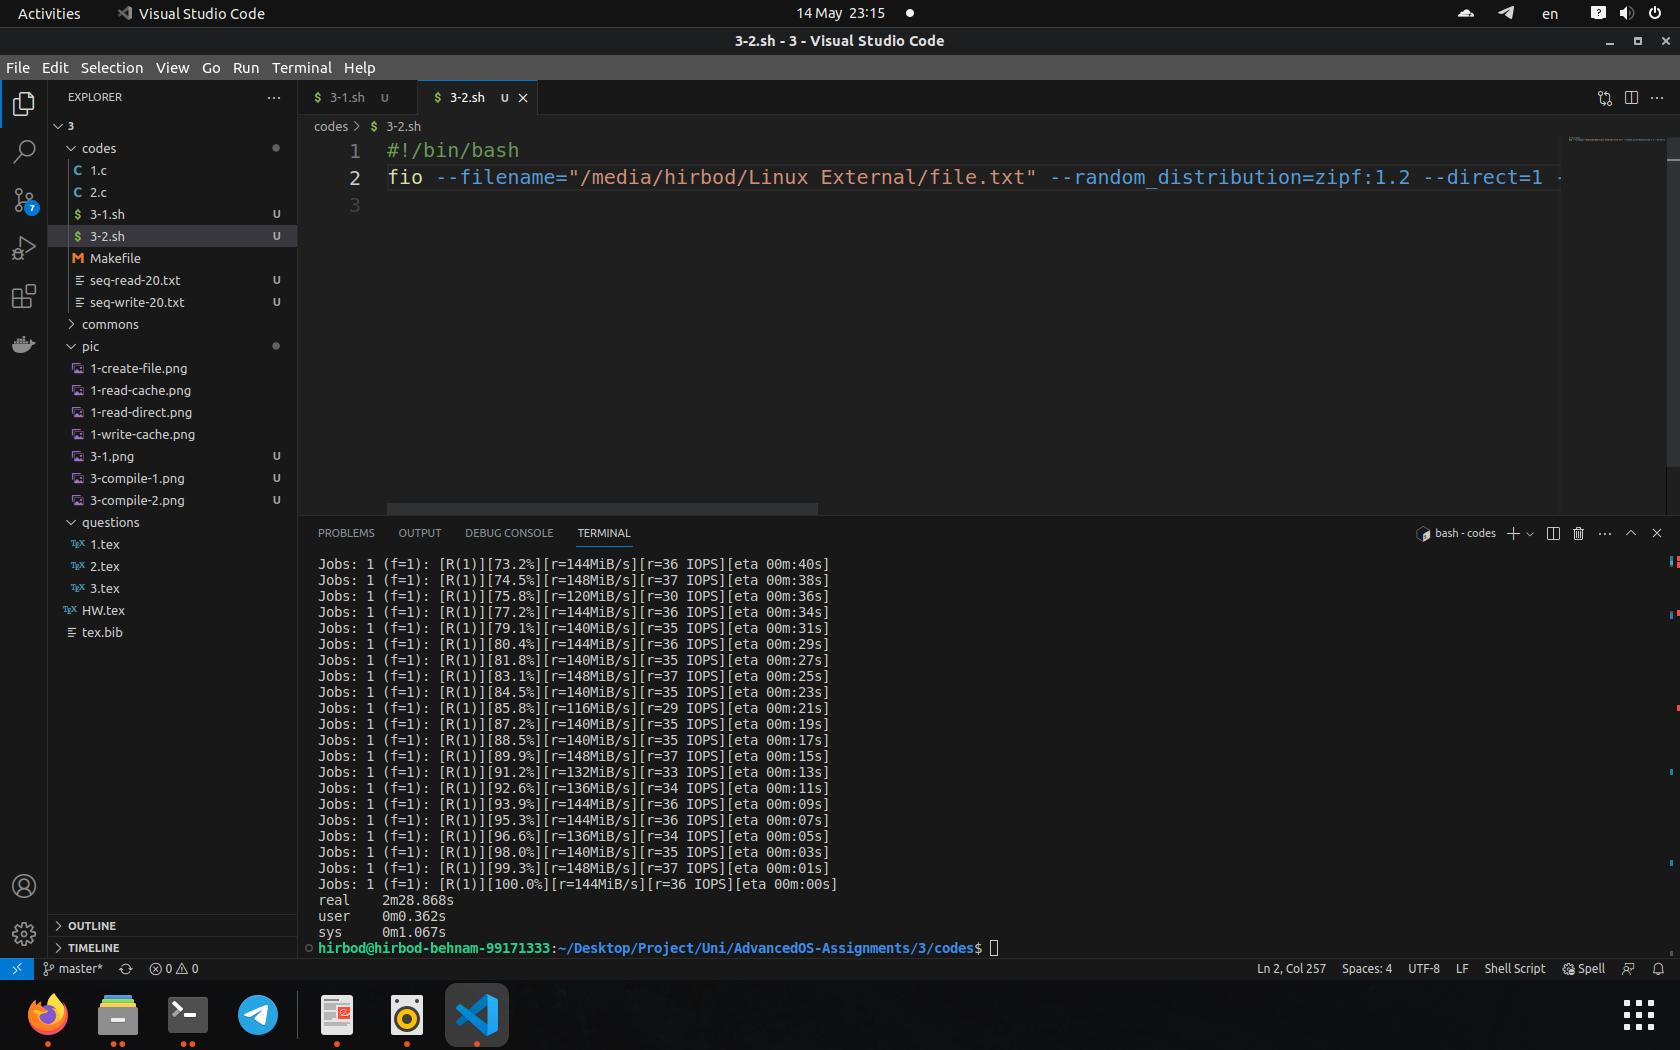
\includegraphics[scale=0.25]{pic/3-2.png}
    \caption{خواندن فایل مستقیم از هارد}
    \label{fig:3-2}
\end{figure}

حال سعی می‌کنیم که از ماژول
\lr{openCAS}
استفاده کنیم. به کمک دستورات زیر می‌توان دیسک جامد را کش برای پارتیشن دیسک سخت کرد.
\samplebox{sudo casadm -S -d /dev/disk/by-id/wwn-0x50026b724c01dd3e-part4 --force -c wt\\
sudo casadm -A -d /dev/disk/by-id/wwn-0x50014ee6058277fa-part8 -i 1}

حال در صورتی که اصلا در
\lr{file explorer}
به قسمت
\lr{computer}
برویم متوجه می‌شویم که یک دیسک جدید اضافه شده است:
\begin{figure}[H]
    \centering
    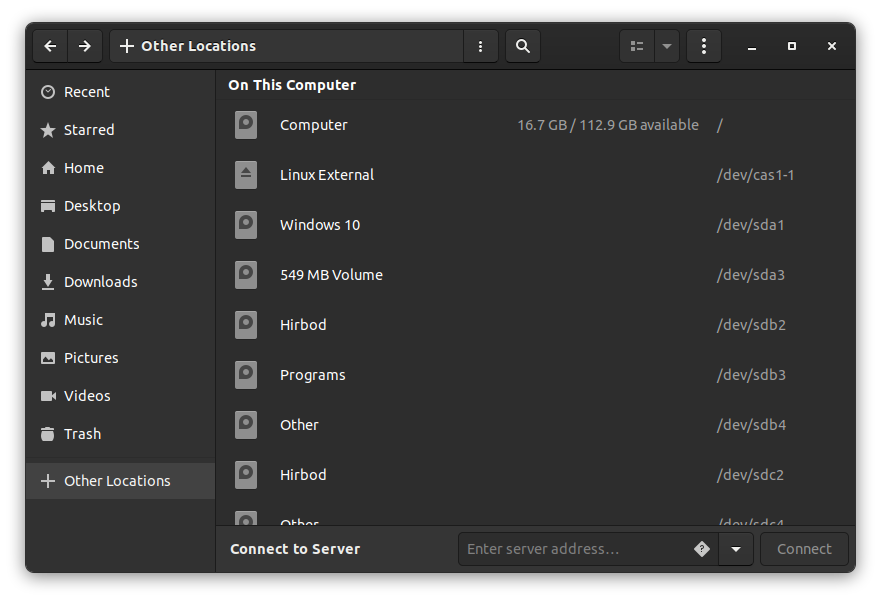
\includegraphics[scale=0.5]{pic/3-cas-nautilus.png}
    \caption{اضافه شدن \lr{CAS} در \lr{file explorer}}
    \label{fig:cas_in_file_explorer}
\end{figure}
در صورتی که بر روی آن کلیک کنیم آن
\lr{mount}
می‌شود. در ابتدا همان طور که در دستورات بالا نیز معلوم است به کمک مود
\lr{write back}
کش را استفاده کردیم. پس شروع به بنجمارک دیسک می‌کنیم. نتایج آن در شکل
\ref{fig:3-4-wt}
آمده است.
\begin{figure}[H]
    \centering
    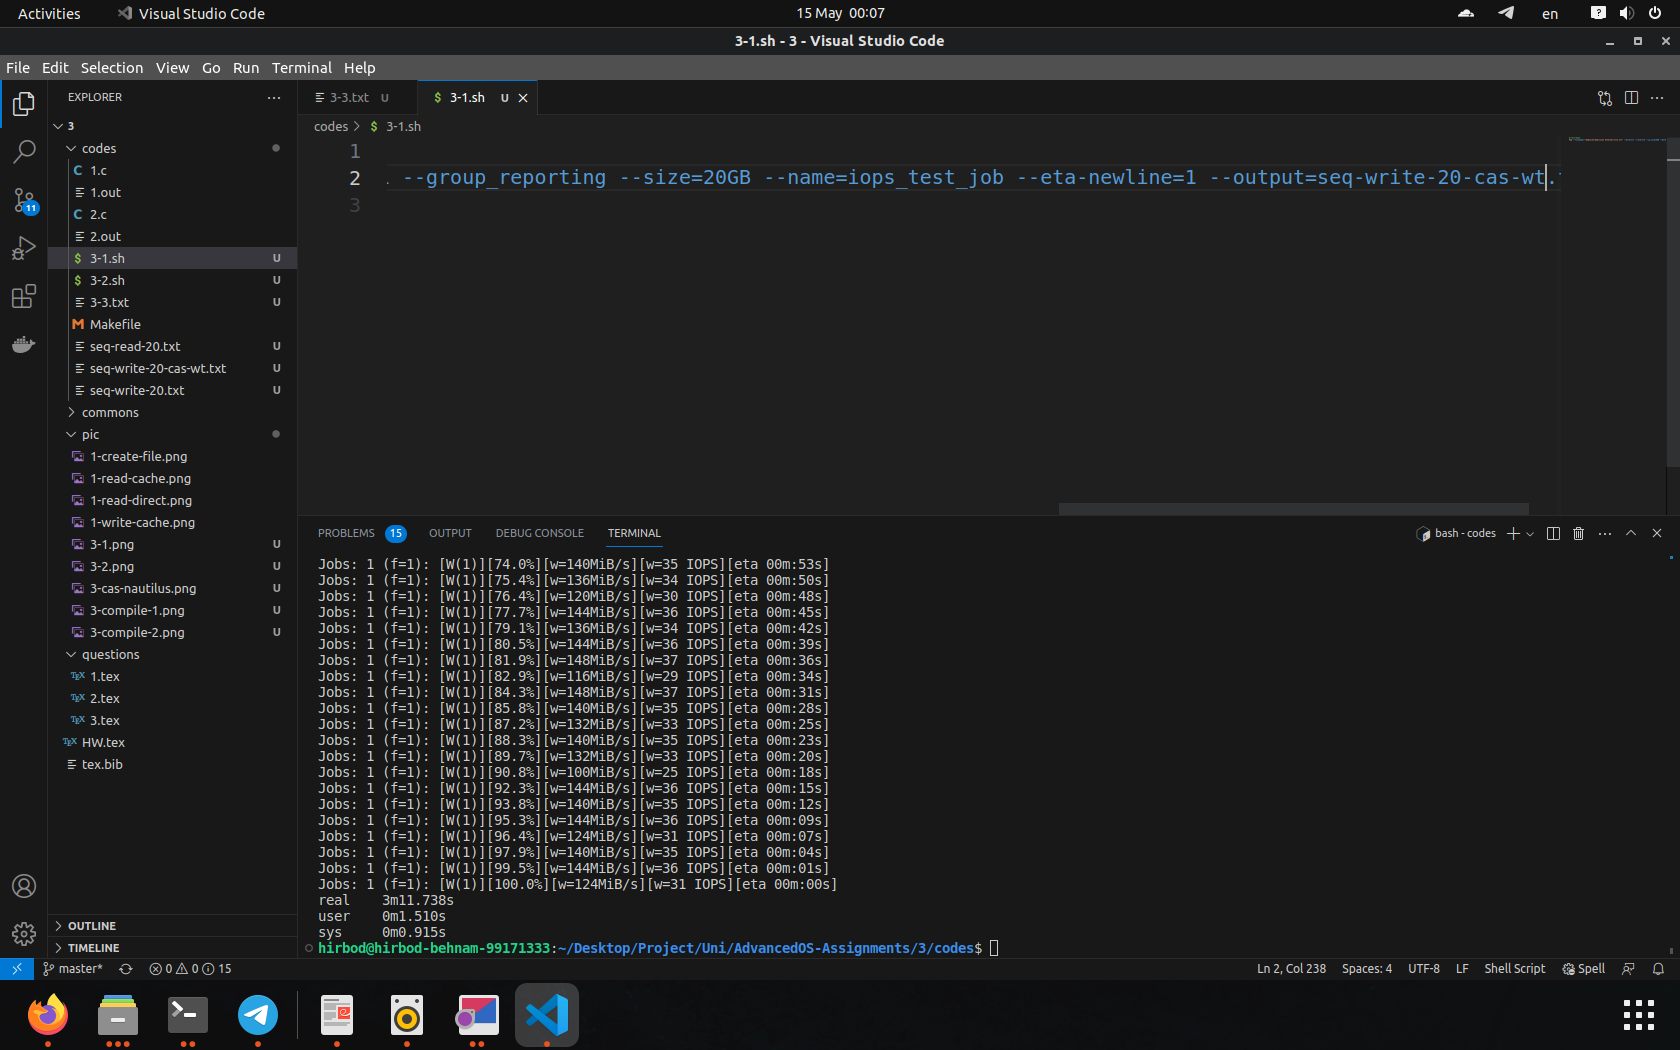
\includegraphics[scale=0.25]{pic/3-wt.png}
    \caption{نوشتن در کش با مود \lr{write through}}
    \label{fig:3-4-wt}
\end{figure}
همان طور که مشخص است کمی سرعت نوشتن کمتر شد! این موضوع احتمالا به دلیل این است که از آنجا که کش ما
\lr{write through}
است اول دیتا در
\lr{SSD}
کش می‌شود و سپس در
\lr{HDD}
نوشته می‌شود. پس منطقی است که در جایی که فقط
\lr{write}
انجام می‌شود سرعت کمی کمتر باشد. سپس تمامی کش‌ها را پاک می‌کنیم به کمک دستورات زیر:
\samplebox{sudo casadm -R -j 1 -i 1\\
sudo casadm -T -i 1}
حال دوباره کش را اینبار با نوع
\lr{write back}
می‌سازیم. نتایج آن در شکل
\ref{fig:3-4-wb}
آمده است.
\begin{figure}[H]
    \centering
    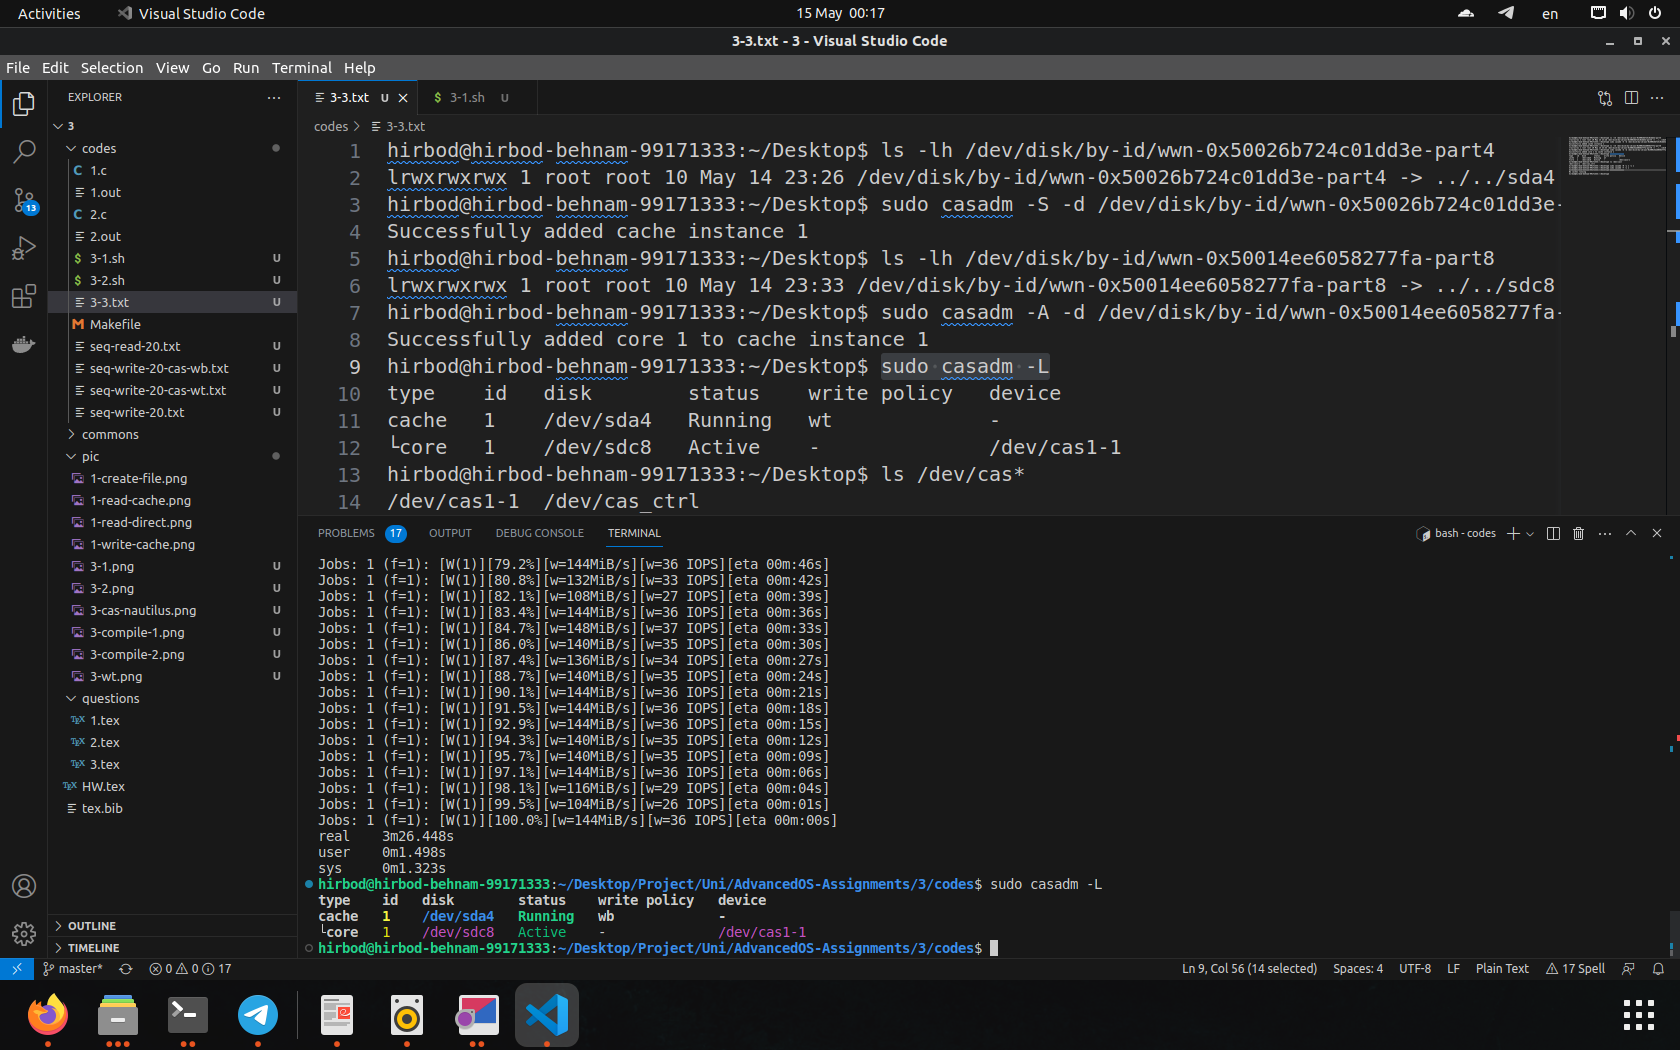
\includegraphics[scale=0.25]{pic/3-wb.png}
    \caption{نوشتن در کش با مود \lr{write back}}
    \label{fig:3-4-wb}
\end{figure}
در این حالت حتی سرعت بدتر از قبل شد! این موضوع به نظرم خیلی عجیب است چرا که حداقل کمی از دیتا باید در کش باقی
می‌ماند. همچنین من دقت کردم زمانی که با سیستم‌عامل کاری نداشتم دیسکم درگیر شد و این موضوع احتمال نشان دهنده‌ی
این است که به مرور زمان
\lr{write back}
انجام می‌شود. شاید دلیل کند بودن این باشد که
\lr{SSD}
من قدیمی
(حدود ۸ سال پیش)
است و سرعت آن کمی کند است
(حدود ۲۵۰ مگابایت بر ثانیه).
شاید برای اینکه در
\lr{workload write}
سرعت را بالا ببریم لازم باشد که از دیسک‌های سریع‌تری استفاده بکنیم.

در نهایت با
\lr{write around}
تست می‌کنیم.
تایج آن در شکل
\ref{fig:3-4-wa}
آمده است.
\begin{figure}[H]
    \centering
    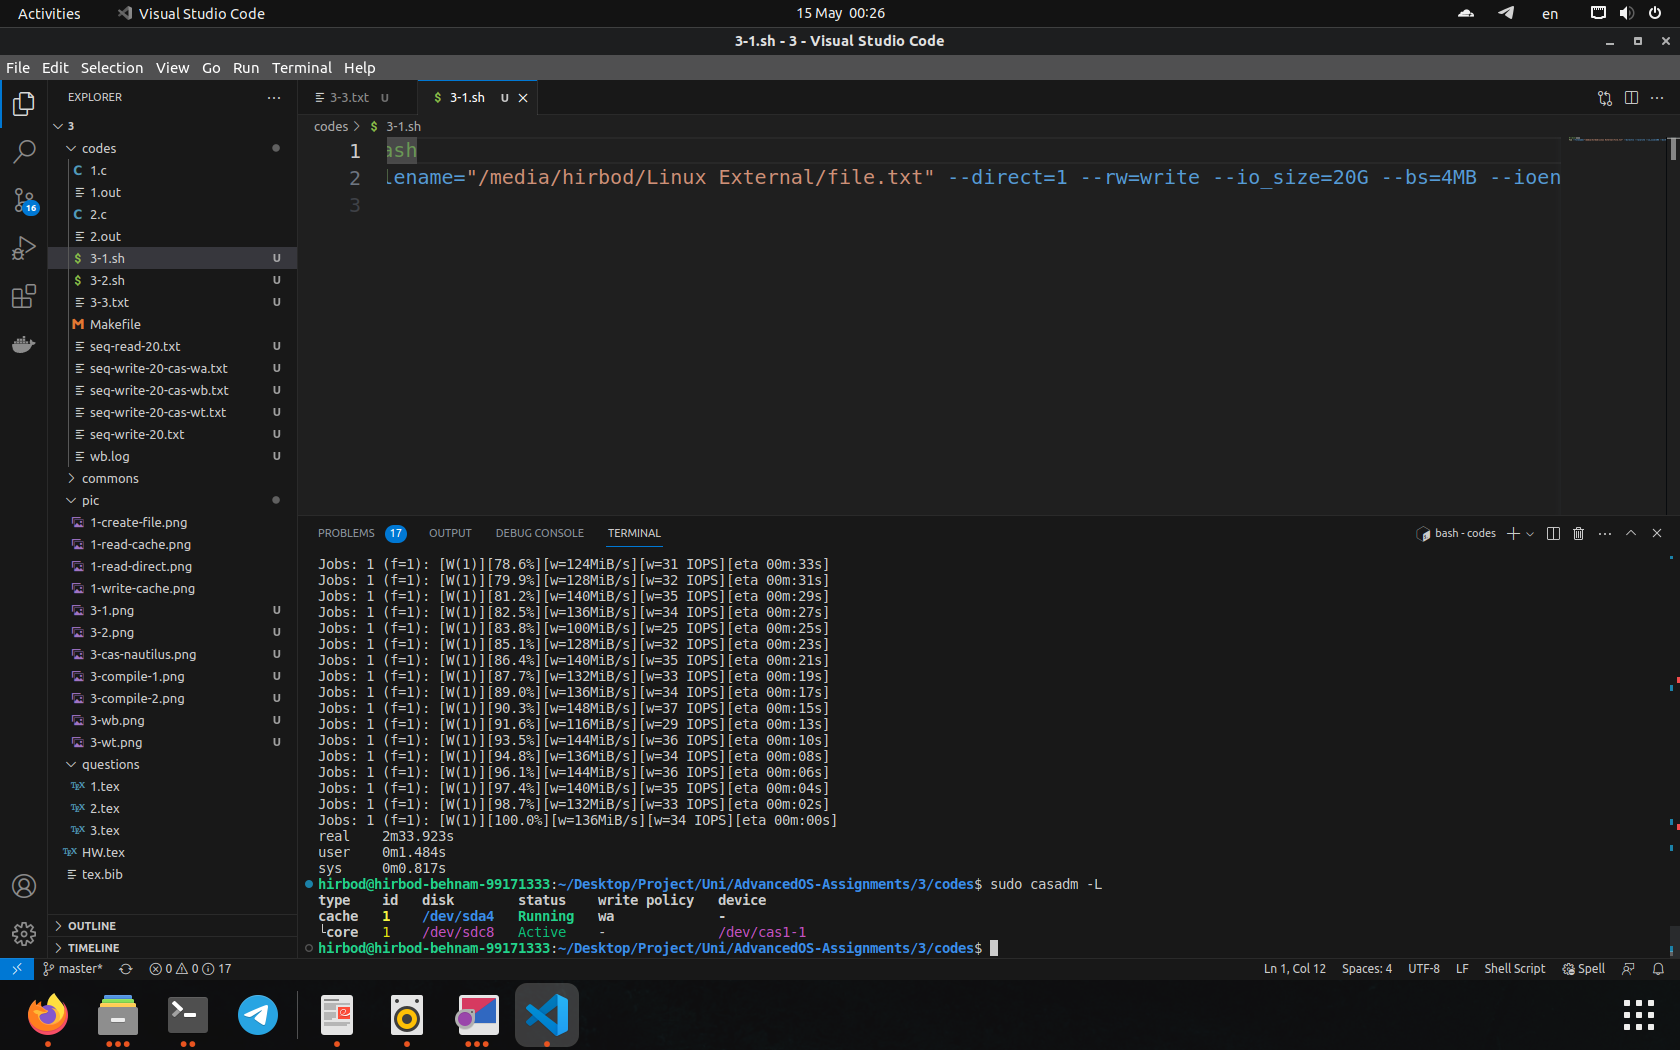
\includegraphics[scale=0.25]{pic/3-wa.png}
    \caption{نوشتن در کش با مود \lr{write around}}
    \label{fig:3-4-wa}
\end{figure}
در این حالت متوجه می‌شویم که سرعت نوشتن تقریبا برابر سرعت نوشتن در
\lr{HDD}
است. برای اینکه بفهمیم این مود دقیقا چیست به
\link{https://open-cas.github.io/cache_configuration.html\#write-around}{داک}
\lr{openCAS}
مراجعه می‌کنیم. با توجه به توضیحات عملا
\lr{write through}
است ولی اگر
\lr{cache line}
وجود نداشته باشد آن لاین را در
\lr{SSD}
نمی‌آورد. به همین دلیل سرعت آن برابر سرعت
\lr{HDD}
شده بود.